Background events can be produced from QED trident processes and wide-angle bremsstrahlung (WAB). The trident processes can be separated into "radiative" and "Bethe-Heitler" diagrams. In particular, the heavy photon production is related to the radiative trident cross section. The $A^{\prime}$ production for a mass bin is described as shown in Equation~\eqref{eq:crossSection}.

\begin{equation}
\label{eq:crossSection}
\dfrac{d\sigma(A'\rightarrow e+e-)}{d\sigma(\gamma*\rightarrow e+e-)} = \left(\dfrac{3\pi\epsilon^{2}}{2N_{eff}\alpha}\right)\left(\dfrac{m_{A'}}{\delta m_{A'}}\right)
\end{equation}

In Equation~\eqref{eq:crossSection}, $N_{eff}$, the number of available decay states, is one for the HPS experiment which explores a mass range in which the heavy photon can only decay to one Standard Model final state ($e+e-$). The $\epsilon^{2}$ refers to the coupling factor between the heavy photon and the Standard Model while the $\alpha$ is the fine structure constant. The $\dfrac{m_{A'}}{\delta_{m_{A'}}}$ refers to the central mass value considered in the mass bin of study. After accounting for all backgrounds, prior to the radiative cut to the data at 80$\%$ of the beam energy, the energy sum of the two particles is in general agreement between Monte Carlo and data as shown in Figure~\ref{fig:mcAgree}.

\begin{figure}[htb]
  \centering
      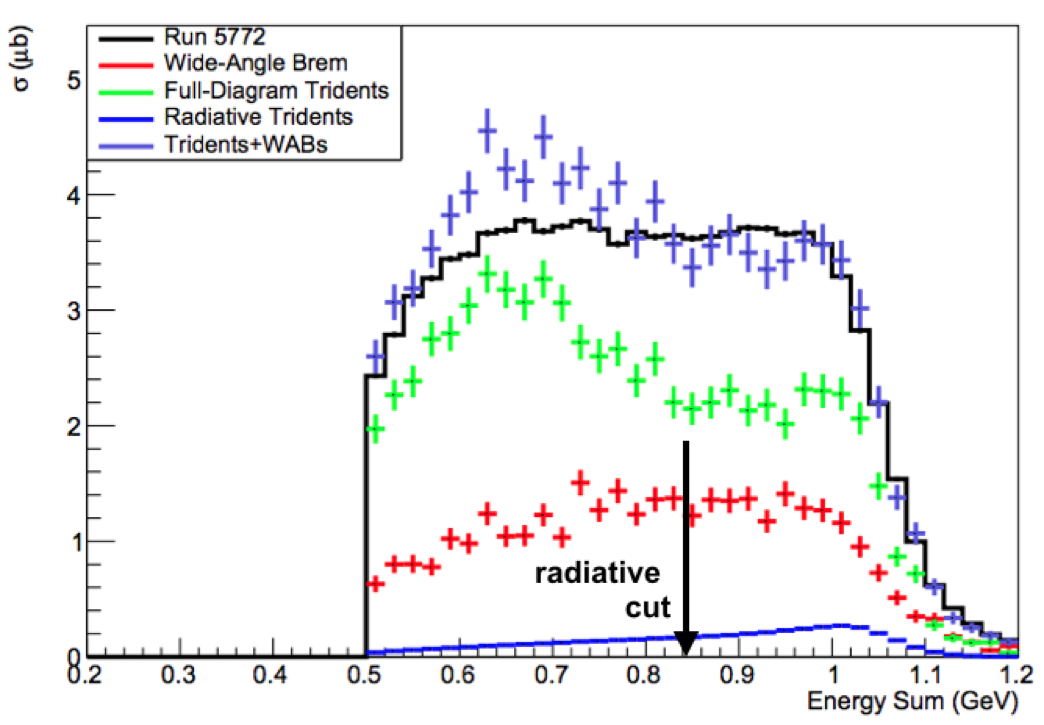
\includegraphics[width=0.8\textwidth]{pics/searching/mcAgree.png}
  \caption[Energy sum comparison in Monte Carlo and data]{Energy sum in Monte Carlo and data. The energy sum is in general agreement at the high end of the spectrum where HPS is optimized to search for heavy photons. Further studies to isolate track and SVT layer inefficiencies at the lower energy sum are still being explored.}
  \label{fig:mcAgree}
\end{figure} 

The fraction of radiative reactions amongst trident events in the HPS search region is the radiative fraction. Using MadGraph5 Monte Carlo to model the tridents and radiatives and MadGraph4 Monte Carlo to model the wide angle bremsstrahlung (WAB) background, the radiative fraction can be determined as shown in Figure~\ref{fig:radFrac}.

\begin{figure}[htb]
  \centering
      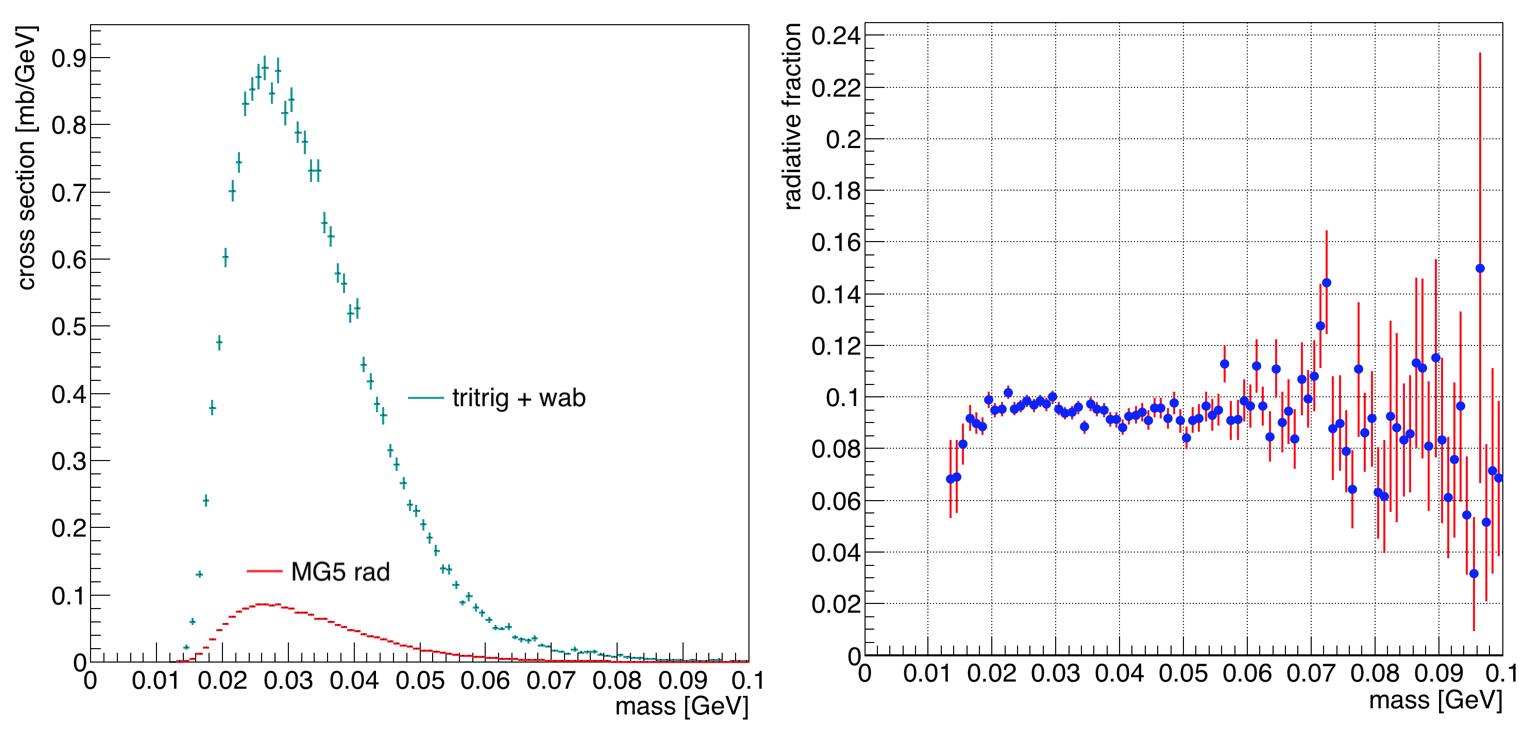
\includegraphics[width=0.9\textwidth]{pics/searching/radFrac.png}
  \caption[Radiative fraction from Monte Carlo]{Radiative fraction using MadGraph5 Monte Carlo and spinfix WAB.}
  \label{fig:radFrac}
\end{figure} 

As shown in Figure~\ref{fig:radFrac}, the radiative fraction relevant to the vertex analysis is approximately 9.5$\%$ for all masses. This fraction is defined as the ratio of radiative events to the background events (tritrig+WAB in Figure~\ref{fig:radFrac}) and is the same for both the 0.5~mm and 1.5~mm data sets.
